\documentclass{standalone}
\usepackage[utf8]{inputenc}
\usepackage{tikz}
\usetikzlibrary{intersections,arrows,calc}
%


\begin{document}

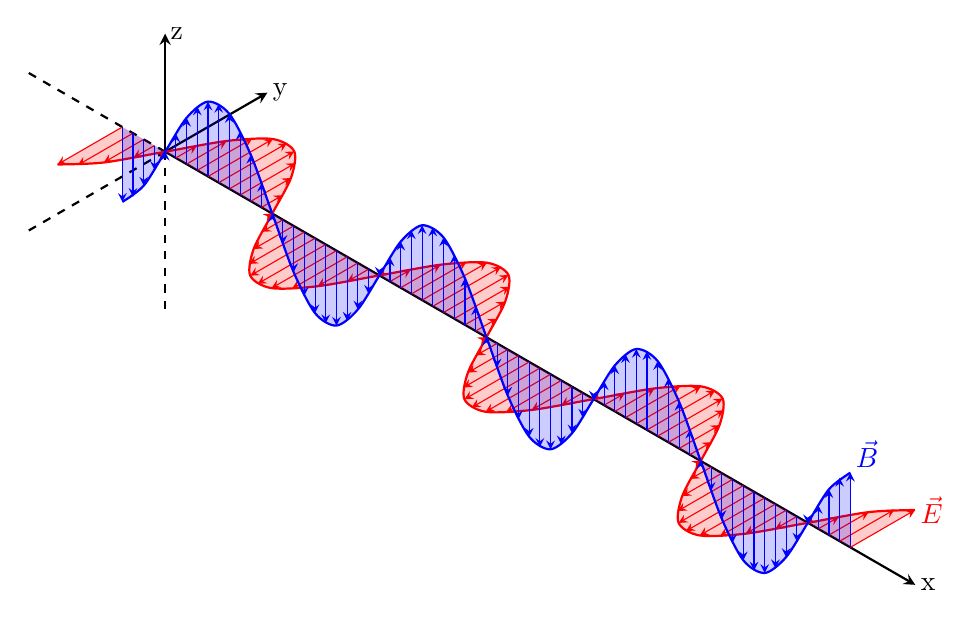
\begin{tikzpicture}
    [x={(0.866cm,-0.5cm)}, y={(0.866cm,0.5cm)}, z={(0cm,1cm)}, scale=1.0,
    %Option for nice arrows
    >=stealth, %
    inner sep=0pt, outer sep=2pt,%
    axis/.style={thick,->},
    wave/.style={thick,color=#1,smooth}];


    % Colors

    \colorlet{lightgreen}{green!80!black};
    \colorlet{darkred}{red!50!black};
    \colorlet{lightred}{red!80!black};

    % Frame
    \coordinate (O) at (0, 0, 0);
    \draw[axis] (O) -- +(11, 0,   0) node [right] {x};
    \draw[axis] (O) -- +(0,  1.5, 0) node [right] {y};
    \draw[axis] (O) -- +(0,  0, 1.5) node [right] {z};
    
    \draw[thick,dashed] (-2,0,0) -- (O);
    \draw[thick,dashed] (0,-2,0) -- (O);
    \draw[thick,dashed] (0,0,-2) -- (O);

    % Electric field vector
    \path[fill=red,opacity=0.2,wave=red, variable=\x,samples at={-0.628,-0.314,...,10.05}]
        plot (\x,{sin(2*\x r)},0) -- (10.05,0,0) -- (-0.628,0,0) -- (-0.628,{sin(-2*0.628 r)},0);
    \draw[wave=red, variable=\x,samples at={-0.628,-0.314,...,10.05}]
        plot (\x,{sin(2*\x r)},0)node[anchor= west]{$\vec{E}$};
    %E field vectors
    \foreach \x in{-.628, -0.471,...,10.05}
        \draw[color=red,->] (\x,0,0) -- (\x,{sin(2*\x r)},0);
        
     % Magnetic field vector
     \path[fill=blue,opacity=0.2,wave=blue, variable=\x,samples at={-0.628,-0.314,...,10.05}]
        plot (\x,0,{sin(2*\x r)}) -- (10.05,0,0) -- (-0.628,0,0) -- (-0.628,0,{sin(-2*0.628 r)});
    \draw[wave=blue, variable=\x,samples at={-0.628,-0.314,...,10.05}]
        plot (\x,0,{sin(2*\x r)})node[anchor=south west]{$\vec{B}$};
    %B field vectors
    \foreach \x in{-.628, -0.471,...,10.05}
        \draw[color=blue,->] (\x,0,0) -- (\x,0,{sin(2*\x r)});    
        
\end{tikzpicture}

\end{document}